% This is samplepaper.tex, a sample chapter demonstrating the
% LLNCS macro package for Springer Computer Science proceedings;
% Version 2.20 of 2017/10/04
%
\documentclass[runningheads]{llncs}
%
\usepackage{cite}
\usepackage{amsmath,amssymb,amsfonts}
\usepackage{algorithmic}
\usepackage{tikz}
\usepackage{pgfplots}
\usepackage{graphicx}
\usepackage{textcomp}
\usepackage{xcolor}
%\usepackage{natbib}

% Used for displaying a sample figure. If possible, figure files should
% be included in EPS format.
%
% If you use the hyperref package, please uncomment the following line
% to display URLs in blue roman font according to Springer's eBook style:
% \renewcommand\UrlFont{\color{blue}\rmfamily}

\begin{document}
%
\title{From Tweets to Token Sales: Assessing ICO Success through Social Media Sentiments}
%
\titlerunning{Assessing ICO Success through Social Media Sentiments}
% If the paper title is too long for the running head, you can set
% an abbreviated paper title here
%

\author{Donghao HUANG\inst{1}\orcidID{0009-0005-6767-4872} \and
SAMUEL\inst{1}\orcidID{0009-0008-2153-8076} \and 
Quoc Toan HUYNH\inst{1}\orcidID{0009-0008-1968-9262} \and
Zhaoxia WANG\thanks{Corresponding Author}\inst{1}\orcidID{0000-0001-7674-5488}}

%
\authorrunning{D. Huang et al.}
%\authorrunning{F. Author et al.}
% First names are abbreviated in the running head.
% If there are more than two authors, 'et al.' is used.
%
\institute{School of Computing and Information Systems, Singapore Management University, 80 Stamford Rd, Singapore 178902, Singapore \\ \texttt{\{dh.huang.2023, samuel1.2021, qthuynh.2020, zxwang\}@smu.edu.sg}}
%

\maketitle              % typeset the header of the contribution
%
\begin{abstract}

With the advent of social network technology, the influence of collective opinions has significantly impacted business, marketing, and fundraising. Particularly in the blockchain space, Initial Coin Offerings (ICOs) gain substantial exposure across various online platforms. Yet, the intricate relationships among these elements remain largely unexplored. This study aims to investigate the relationships between social media sentiment, engagement metrics, and ICO success. We hypothesize a positive correlation between favorable sentiment in ICO-related tweets and overall project success. Additionally, we recognize social media engagement indicators (mentions, retweets, likes, follower counts) as critical factors affecting ICO performance. Employing machine learning techniques, we conduct sentiment analysis on tweets, discerning emotional nuances and categorizing expressions as positive or negative. Employing established classification methods, we further analyze engagement data to reveal its impact on ICO interest and awareness. Our research findings offer insights into the predictive potential of social media strategies for ICO success and underscore the importance of investor sentiment and engagement in the volatile cryptocurrency landscape. These insights provide actionable guidance for aspiring crypto founders in formulating effective business development strategies. 


The source codes and datasets of this paper are accessible at GitHub: https://github.com/inflaton/Success-Indicators-of-Initial-Coin-Offerings

\keywords{Cryptocurrency \and Initial Coin Offerings(ICOs) \and Sentiment analysis \and Social media \and Machine Learning }

\end{abstract}



\section{Introduction}

The emergence of blockchain technology and cryptocurrencies has transformed fundraising through methods like Initial Coin Offerings (ICOs) and Initial Exchange Offerings (IEOs) \cite{campino2021initial}. ICOs, also known as token sales, provide cost-effective fundraising avenues by issuing new coins on blockchain-based platforms. Social media platforms, particularly Twitter, have significantly contributed to the promotion and dissemination of information about both ICOs and IEOs \cite{tiwari2020future}.

IEOs, facilitated by cryptocurrency exchanges, involve these platforms managing fundraising campaigns by issuing new tokens \cite{chamorro2021financing}. Acting as intermediaries between projects and investors, these exchanges offer comprehensive crowd sale services \cite{vivion2020supporting}. The ICO model witnessed substantial funding, with 3,782 ICOs launched in 2018 alone, collectively raising nearly \$11.4 billion \cite{boreiko2019new}, \cite{giudici2019impact}. Despite fluctuations, the prevalence of ICOs persisted in 2021, with 113 hosted on Coincodex \cite{giudici2019impact}, \cite{daskalakis2020introduction}. The foundation of an ICO rests on its whitepaper, outlining project details such as business strategy, token sale structure, fund allocation, team composition, and development roadmap \cite{daskalakis2020introduction}. Utilizing the broad reach of social media, ICOs frequently leverage platforms like Twitter to promote their offerings within the crypto community \cite{drobetz2019investor}.

Businesses utilize Airdrop initiatives to increase awareness about emerging ICOs or IEOs, rewarding participants with digital tokens or cryptocurrency for engaging in marketing activities. This involves actions like joining Telegram groups, following on social media platforms, retweeting, and tagging friends, fostering community engagement and brand endorsement \cite{howell2020initial}. Social media, especially Twitter, plays a vital role in the success of ICOs and IEOs, offering swift, cost-effective means to raise capital, supported by blockchain's efficiency in creating digital tokens through smart contracts, ensuring security and reliability \cite{morkunas2019blockchain}.

Existing studies on ICOs and IEOs often focus solely on direct social media mentions, neglecting the potential impact of indirect interactions. This study aims to bridge this gap by comprehensively analyzing both direct and indirect social media interactions related to crypto projects. It explores sentiment and engagement levels in direct tweets, replies mentioning token keywords, and project announcements on Twitter. By predicting ICOs success using social media sentiment and engagement, this study seeks to uncover their interrelation, offering insights into the factors influencing ICOs and IEOs success on social media.


The main contributions of this paper are summarized as follows:
\begin{enumerate}
    \item The study delves into the intricate relationships among social media, such as Tweets, and ICO success in the blockchain space, which remains largely unexplored. This contributes to filling the gap in understanding how these elements interact and influence each other.
    
     \item By employing machine learning techniques for social media sentiment analysis and analyzing engagement data, the research aims to reveal the predictive potential of social media strategies for ICO success. This contribution offers valuable insights for crypto founders, indicating the importance of effective social media utilization in driving project success.
     
    \item The research findings offer actionable guidance for aspiring crypto founders by emphasizing the significance of investor sentiment and engagement in the volatile cryptocurrency landscape. This contribution provides practical advice for formulating effective business development strategies in the blockchain industry.
\end{enumerate}


%The source codes and datasets of this paper are accessible at GitHub %\footnote{\url{https://github.com/inflaton/Success-Indicators-of-Initial-Coin-Offerings}}.

\section{Related Work \& Motivations}
ICOs have become a popular means for startups to raise funds. However, the success of ICOs is influenced by various factors that need to be considered for a comprehensive understanding of their fundraising outcomes. 

As social media platforms continue to evolve, there has been a notable surge in individual and organizational engagement, with a growing emphasis on expressing and sharing opinions~\cite {fu2013social,chen2020comparing}. Consequently, social media sentiment analysis has garnered widespread popularity~\cite {wang2014enhancing,wang2023mimusa,teo2023knowledge}. Such sentiment analysis of social media serves as a vital method for individuals and organizers facilitating a deeper understanding of prevailing opinions and sentiments~\cite {wang2014anomaly,wang2014issues,hu2023msrl,wang2023learning}, thereby aiding  decision-making processes crucial for business success.


Social media sentiment analysis has become indispensable in the financial domain, supported by numerous studies highlighting its effectiveness and contributions~\cite{wang2018stock,hu2021stock,wang2023learning}. While these studies have identified various predictors of success, Campino et al. stress the necessity for a more comprehensive analysis of social media's evolving role in ICO outcomes~\cite{campino2021success}. Despite identifying key predictors such as third-party ratings and detailed whitepapers, the study lacks depth in exploring the multifaceted influence of social media on ICO performance.

%We contend that a deeper examination of social media dynamics is essential for a comprehensive understanding of ICO success factors and for informing strategic decision-making in this rapidly evolving landscape.

Some researchers have underscored the importance of factors such as detailed project information, idea uniqueness, and team competencies \cite{alchykava2021ico}. Yet, they often overlook the significant influence of social media on investor behavior. 
Another study identified conditions to enhance ICO credibility, including registration, GitHub code publication, and early funding \cite{belitski2022success}. However, this overlooks potential drawbacks such as the effort required to secure funding and risks associated with code transparency.

In a separate analysis, Lyandres et al. identified various ICO success factors, including hardcap, whitepaper informativeness, pre-ICO social media activity, bonuses, and transparency \cite{lyandres2020ico}. However, its limited time scope and lack of consideration for negative sentiment impact are notable limitations.

Twitter sentiment analysis plays a pivotal role in evaluating ICO effectiveness \cite{albrecht2020behavior}. The platform's global reach facilitates succinct communication, fostering high engagement rates \cite{mohd2020liability}. Analyzing meticulously collected Twitter comments related to ICOs, sentiment analysis unveils behavioral and social sentiment patterns among investors. These insights serve as a foundation for devising effective marketing strategies \cite{calderwood2019travel}.


Influencer-driven product tweets significantly influence brand trust and consumer decisions. Twitter discussions bolster brand recognition and attract new audiences, leading to increased sales \cite{appel2020future}. Our study aims to comprehensively explore global social media strategies' impact on ICO success, contrasting with regional studies \cite{chursook2022twitter}. Understanding social media's influence aids startups in refining marketing strategies and engaging with investors. Analyzing social media metrics and sentiment guides effective investor targeting and platform selection for ICO promotion. A holistic social media study offers invaluable insights for ICO fundraising efforts.


% \subsection{Maintaining the Integrity of the Specifications}

\section{Hypotheses}
Hypothesis 1: Positive sentiment expressed in tweets mentioning an ICO is correlated with its success. Sentiment analysis of tweets can provide valuable insights into public perception of a cryptocurrency project. The NRC Word-Emotion Association Lexicon can be used to analyse the emotional content of tweets and identify positive and negative sentiments. A higher proportion of positive tweets is likely to indicate a successful ICO. Sentiment analysis can be performed by collecting and analyzing tweets mentioning the ICO and their respective replies. Table \ref{tab1} illustrates some examples of original and reply tweet data that were used for the analysis.

\begin{table}[htbp]
\caption{Example of data used for sentiment analysis.}
\begin{center}
\begin{tabular}{|c|c|c|}
\hline
 & \textbf{Tweet Content} & \textbf{Sentiment} \\
 \hline
Original Tweet & Just bought more \$SOL, & Positive \\
& feeling great about this investment!! & \\
\hline
Reply & I'm not convinced,  & Negative \\
& I think \$SOL is overvalued & \\
\hline
Reply & Quite bullish on it too,  & Positive \\
&the fundamentals are really strong& \\
\hline
Reply & Waiting to see how the market  & Negative \\
& develops, but currently looking for & \\
&  better options in the market & \\
\hline
\end{tabular}
\label{tab1}
\end{center}
\end{table}

Hypothesis 2: The level of engagement on social media, such as the number of mentions, retweets, likes, and followers, is positively associated with the success of an ICO. Engagement on social media can indicate the level of awareness and interest in a cryptocurrency project among potential investors. By collecting data on the number of mentions, retweets, likes, and followers of the project and the users mentioning it, we can measure the level of engagement and use it to predict the success of an ICO. Table \ref{tab2} illustrates an example of the engagement metrics used, and the number of each metric collected for the \$MATIC crypto token.

\begin{table}[htbp]
\caption{Example of data used for engagement metrics.}
\begin{center}
\begin{tabular}{|c|c|}
\hline
\textbf{Metric} & \textbf{Data collected for \$MATIC} \\
\hline
Number of mentions & 799,849 \\
\hline
Number of retweets & 1,471,118 \\
\hline
Number of likes & 1,280,414 \\
\hline
Number of project followers & 34,755,686 \\
\hline
\end{tabular}
\label{tab2}
\end{center}
\end{table}

\section{Dataset}

ICOs data was collected from iconbench\footnote{\url{www.icobench.com}} and cryptoran\footnote{\url{www.cryptorank.io}} using a combination of manual download and automatic scraping using Python beautiful soup package\footnote{\url{https://beautiful-soup-4.readthedocs.io/}}. For each cryptocurrency project, we recorded ICO-related data as summarized in Table \ref{tab3}.

\begin{table}[htbp]
\caption{ICO data collected.}
\begin{center}
\begin{tabular}{|c|c|c|}
\hline
\textbf{Data description} & \textbf{Data type} & \textbf{Hypothesis} \\
\hline
Project name & String & 1, 2 \\
\hline
Project token & String & 1, 2 \\
\hline
Soft cap & Integer & 1, 2 \\
\hline
Total raised & Integer & 1, 2 \\
\hline
ICO Date & Date & 1, 2 \\
\hline
\end{tabular}
\label{tab3}
\end{center}
\end{table}


Data from Twitter was gathered using the Twitter API and Scrapy\footnote{\url{https://scrapy.org/}}, an open-source Python framework. The collection encompassed two categories of tweets: those that included a cryptocurrency project's keyword, marked by the prefix ``\$'' followed by the token's name (e.g., ``\$SOL'' or ``\$MATIC''), and tweets emanating from the project's official Twitter handle. For tweets featuring the token keyword, we compiled data on the number of retweets, likes, and the poster's follower count, in addition to the content of any responses. However, tweets originating from the project’s own account were excluded from direct analysis as they primarily represent official communications from the cryptocurrency project's team, thus deemed not directly pertinent to the research hypotheses.


Tweets are categorized into direct mentions and indirect mentions. A direct mention occurs when a tweet explicitly contains the token keyword. An indirect mention refers to a tweet that either responds to another tweet featuring the token keyword or replies to a tweet from the project's official Twitter handle. It's important to highlight that to avoid look-ahead bias, only tweets published prior to the dates of a token's ICO are considered relevant for assessing the ICO's prospective success.

After collecting the above data, we processed and transformed it to obtain useful information. For each cryptocurrency project, we recorded the following twitter data as summarized in Table \ref{tab4}:

\begin{table}[htbp]
\caption{Twitter data collected.}
\begin{center}
\begin{tabular}{|c|c|c|}
\hline
\textbf{Data description} & \textbf{Data type} & \textbf{Hypothesis} \\
\hline
Content of tweets - direct mentions & List of String & 1 \\
\hline
Content of tweets - indirect mentions & List of String & 1 \\
\hline
Total number of direct mentions & Integer & 2 \\
\hline
Total number of indirect mentions & Integer & 2 \\
\hline
Total number of likes & Integer & 2 \\
\hline
Total number of retweets & Integer & 2 \\
\hline
Number of official account followers & Integer & 2 \\
\hline
Total number of followers of  & Integer & 2 \\
users mentioning project && \\
\hline
\end{tabular}
\label{tab4}
\end{center}
\end{table}

\section{Experiment \& Methodology}

\subsection{Data Processing}
%To better cater to machine learning models used in investigating the two proposed hypotheses, we processed and transformed the data into trainable formats.

For the facilitation of machine learning algorithms in the examination of our hypotheses, data preprocessing was undertaken to convert the raw data into a format amenable to algorithmic training.


Sentiment analysis was a pivotal component of our study, aimed at capturing the emotional undercurrents embedded in both overt and covert mentions. This was achieved by leveraging the NRC Word-Emotion Association Lexicon\footnote{\url{https://saifmohammad.com/WebPages/NRC-Emotion-Lexicon.htm}}, a compendium that assigns sentiments—either positive or negative—to various words. We utilized TextBlob\footnote{\url{https://textblob.readthedocs.io/}}, a Python library recognized for its simple API that enables execution of several natural language processing (NLP) tasks, including sentiment analysis. This was instrumental in quantifying the sentiment polarity of each tweet. Figure \ref{fig1} provides a visual representation of the sentiment evaluation conducted on tweets pertaining to the DUO Network (DUO) ICO.

\begin{figure}[htbp]
\centering
\resizebox{0.5\textwidth}{!}{%
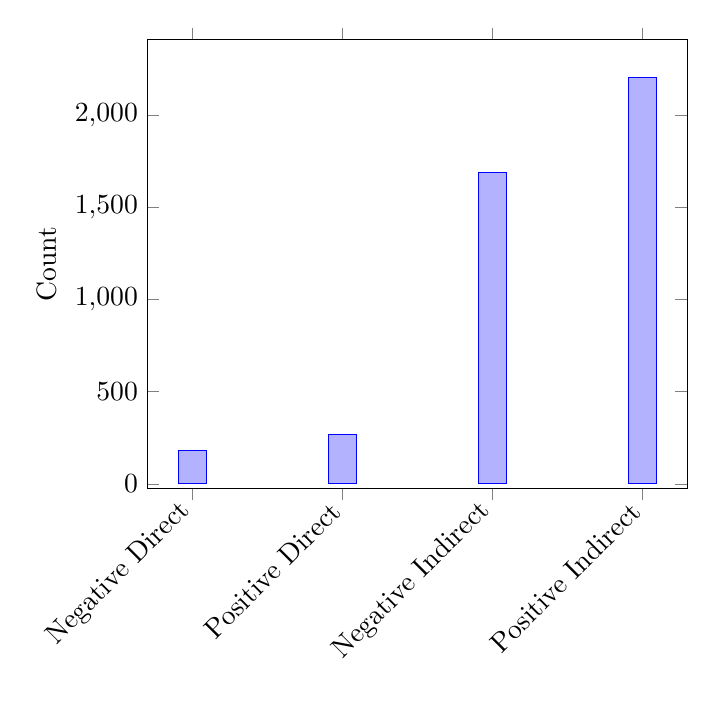
\begin{tikzpicture}
% \begin{axis}[
% 	x tick label style={
% 		/pgf/number format/1000 sep=},
% 	ylabel=Count,
% 	enlargelimits=0.05,
% 	legend style={at={(0.5,-0.1)},
% 	anchor=north,legend columns=-1},
% 	ybar interval=0.7,
% ]

\begin{axis}[ybar, symbolic x coords = {Negative Direct, Positive Direct, Negative Indirect, Positive Indirect}, xtick = data, ylabel = Count, x tick label style={rotate=45,anchor=east}]
\addplot 
	coordinates {(Negative Direct, 180) (Positive Direct, 266)
		 (Negative Indirect, 1689) (Positive Indirect, 2208)};
\end{axis}
\end{tikzpicture}
}%
\caption{Sentiment scores for DUO Network (DUO) tweets.}
\label{fig1}
\end{figure}



The success of an ICO was quantitatively determined by comparing the total capital raised against the soft cap defined by the project, with the latter serving as the minimum required funding level. In our corpus of 816 ICOs, 582 were classified as having achieved success by surpassing their respective soft caps, whereas 234 were deemed unsuccessful for not meeting these financial benchmarks. The dataset was structured into 12 columns, each representing a discrete attribute of an ICO from a specific cryptocurrency project. A condensed overview of these attributes is delineated in Table \ref{tab5}, which can be found in the Appendix.

\subsection{Machine Learning Methods}

The objective of the current research was to forecast the potential success of Initial Coin Offerings (ICOs) by categorizing them as likely to succeed or not. This was based on an array of input variables, all represented by integer values, including attributes like 'soft\_cap', 'total\_positive\_direct\_mentions', among others. We segmented the data into two distinct groups: one for training, constituting 80\% of the entire dataset, and the other for testing, making up the remaining 20\%. Our methodological approach encompassed the deployment of six diverse algorithms, specifically Support Vector Machines (SVMs), Logistic Regression, Random Forest, Naïve Bayes, Categorical Boosting (CatBoost), and Neural Network. These methods were selected for their proven competency in executing classification tasks. The process of parameter optimization was conducted through grid search with the aim of maximizing accuracy.




\section{Results \& Discussion}

\subsection{Individual hypothesis testing}
The classification methods were first applied to hypothesis 1 - ``Positive sentiment expressed in tweets mentioning an ICO is correlated with its success'' by using only the x variables directly linked to sentiments (variables 2, 3, 5, 6 in Table \ref{tab5}). Table \ref{tab6} illustrates the performance outcomes of each predictive model. 

%A comparison with existing model built on local sentiment(11) is shown in figure 2. 

\begin{table}[htbp]
\caption{Hypothesis 1 predictive results}
\begin{center}
\begin{tabular}{|c|c|c|c|c|}
\hline
\textbf{Model} & \textbf{Accuracy} & \textbf{Precision} & \textbf{Recall} & \textbf{F1 Score} \\
\hline
Naïve Bayes & 65.9\% & 66.0\% & 98.1\% & 78.9\% \\
\hline
SVM & 65.2\% & 65.2\% & \textbf{100.0\%} & 79.0\% \\
\hline
Logistic Regression & 66.5\% & \textbf{81.7\%} & 62.6\% & 70.9\% \\
\hline
Random Forest & 73.8\% & 75.4\% & 88.8\% & 81.5\% \\
\hline
CatBoost & 73.8\% & 75.4\% & 88.8\% & 81.5\% \\
\hline
Neural Network & \textbf{74.4\%} & 76.0\% & 88.8\% & \textbf{81.9\%} \\
\hline
\end{tabular}
\label{tab6}
\end{center}
\end{table}

%\begin{figure}[htp]
%    \centering
%    \includegraphics[width=10cm]{table_5-relatedworks}
%    \caption{Comparison to Related Works (11)}
%    \label{fig:relatedworks}
%\end{figure}

Next, the same methods were applied to hypothesis 2 - ``The level of engagement on social media, such as the number of mentions, retweets, likes, and followers, is positively associated with the success of an ICO'' by using the remaining variables which are directly linked to level of engagement. Table \ref{tab7} presents the performance outcomes for each predictive model.

%A comparison with existing model built on expert opinion (11) is shown in figure 3.

\begin{table}[htbp]
\caption{Hypothesis 2 predictive results}
\begin{center}
\begin{tabular}{|c|c|c|c|c|}
\hline
\textbf{Model} & \textbf{Accuracy} & \textbf{Precision} & \textbf{Recall} & \textbf{F1} \\
\hline
Naïve Bayes & 64.6\% & 65.4\% & 97.2\% & 78.2\% \\
\hline
SVM & 65.2\% & 65.2\% & \textbf{100.0\%} & 79.0\% \\
\hline
Logistic Regression & 65.2\% & \textbf{82.9\%} & 58.9\% & 68.9\% \\
\hline
Random Forest & \textbf{76.8\%} & 78.0\% & 89.7\% & \textbf{83.5\%} \\
\hline
CatBoost & 76.2\% & 76.6\% & 91.6\% & 83.4\% \\
\hline
Neural Network & 73.8\% & 76.2\% & 86.9\% & 81.2\% \\
\hline
\end{tabular}
\label{tab7}
\end{center}
\end{table}
%\begin{figure}[htp]
%    \centering
%    \includegraphics[width=10cm]{table_6-relatedworks}
%    \caption{Comparison to Related Works (11)}
%    \label{fig:relatedworks}
%\end{figure}

The results shown in Table \ref{tab6} suggest that the models trained to test Hypothesis 1 yielded moderate performance scores, with the highest accuracy achieved by the Neural Network model at 74.4\%. The F1 Scores ranged from 70.9\% to 81.9\%, which is moderately high. These results indicate that Hypothesis 1 has some merit and performs decently in predicting the success of ICOs based on positive sentiment expressed in tweets.

In contrast, the models trained to test Hypothesis 2 in Table \ref{tab7} performed better overall, with the highest accuracy achieved by the Random Forest model at 76.8\%. The Precision and Recall scores for all models were relatively high, ranging from 65.2\% to 82.9\% for Precision and 58.9\% to 100.0\% for Recall, respectively. The F1 Scores ranged from 68.9\% to 83.5\%, which is slightly higher than the accuracy/F1 scores achieved in the models trained to test Hypothesis 1. These results suggest that while sentiment expressed through tweets may be a moderately strong predictor of ICO success (hypothesis 1), the level of engagement a crypto project has on social media might act as a better predictor (hypothesis 2), supporting the plausibility of hypothesis 2 over hypothesis 1.

\subsection{Combined hypotheses testing}
A combination of the feature sets from both hypotheses was tested for predictive power. This appeared to improve the overall performance, particularly for the CatBoost model, as seen in Table \ref{tab8}. 
%A comparison with existing model built on local sentiment and expert opinion is shown in figure 4.

\begin{table}[htbp]
\caption{Combined predictive results}
\begin{center}
\begin{tabular}{|c|c|c|c|c|}
\hline
\textbf{Model} & \textbf{Accuracy} & \textbf{Precision} & \textbf{Recall} & \textbf{F1} \\
\hline
Naïve Bayes & 64.0\% & 65.2\% & 96.3\% & 77.7\% \\
\hline
SVM & 65.2\% & 65.2\% & \textbf{100.0\%} & 79.0\% \\
\hline
Logistic Regression & 64.6\% & 85.5\% & 55.1\% & 67.0\% \\
\hline
Random Forest & \textbf{78.0\%} & \textbf{79.3\%} & 89.7\% & 84.2\% \\
\hline
CatBoost & \textbf{78.0\%} & 77.1\% & 94.4\% & \textbf{84.9\%} \\
\hline
Neural Network & 67.1\% & 66.5\% & \textbf{100\%} & 79.9\% \\
\hline
\end{tabular}
\label{tab8}
\end{center}
\end{table}
%\begin{figure}[htp]
%    \centering
%    \includegraphics[width=10cm]{table_7-relatedworks}
%    \caption{Comparison to Related Works (11)}
%    \label{fig:relatedworks}
%\end{figure}
%The performance of the proposed model seems to be lacking in comparison to the related work's. This could be due to the difference in taking global data compared to local data only. 

%Overall, the results suggest that both Hypothesis 1 and 2 may have value in predicting the success of ICOs, especially when used together. The CatBoost model performed the best overall in terms of accuracy.

The findings indicate that both Hypothesis 1 and Hypothesis 2 could be effective in forecasting ICO success, particularly when applied in conjunction. Among the tested models, CatBoost and Random Forest emerged as the top performers in accuracy.

\subsection{Further Discussion}

There are several potential reasons why the level of engagement on social media may be a more reliable predictor of the success of an ICO than positive sentiment expressed in tweets. One reason is that the level of engagement on social media is a more comprehensive measure of interest and support for a project, considering factors such as the number of mentions, retweets, likes, and followers \cite{albrecht2019sentiment}. Positive sentiment expressed in tweets, on the other hand, may not capture all forms of engagement and may be influenced by factors such as bots and fake accounts \cite{mirtaheri2021identifying}.

Furthermore, the sentiment expressed in tweets may not always reflect the true feelings and opinions of the wider community \cite{fi12030060}. For example, some people may not reply to tweets or publicly express their support or interest in a project, but may still be engaged with the project on other levels, such as following its social media pages or participating in ICOs and purchasing the tokens without posting anything on Twitter. In contrast, the level of engagement on social media provides a more comprehensive and holistic view of the level of interest and engagement in a project.

Another potential reason why positive sentiment expressed in tweets may not be as strong an indicator of success as the level of engagement on social media is that sentiment can be influenced by a variety of factors, including competitors, influencers, and external events. For example, a project that is in direct competition with another project may receive a high volume of negative sentiment simply because of the rivalry, even if the project itself is strong and has potential for success. Therefore, sentiment expressed in tweets may not always accurately reflect the actual quality and potential of a project.

Another point to consider is that negative sentiment expressed on social media can sometimes have unintended positive effects. In the age of information overload, negative tweets or comments may grab more attention than positive ones and can generate buzz and discussion around a project, leading to increased visibility and exposure \cite{freeman2018enhancing}. It is also important to note that bad marketing is still marketing, and negative sentiment can still create awareness and interest in a project. Therefore, when evaluating the potential success of a project, it is essential to consider both positive and negative sentiment expressed on social media. While positive sentiment is a good indicator of potential success, it should not be the sole metric to evaluate a project, as it can be influenced by external factors such as competitors or influencers. Ultimately, a more comprehensive view of sentiment and engagement on social media is necessary to accurately evaluate the potential success of a project.

Overall, the level of engagement on social media appears to be a more reliable predictor of the success of an ICO than positive sentiment expressed in tweets. The comprehensive and holistic nature of engagement metrics such as mentions, retweets, likes, and followers, combined with their relative independence from external factors such as competition and sentiment, make them a more robust and reliable measure of interest and support for a project.

Our findings highlight the crucial role of social media engagement in predicting ICO success, suggesting a strategic focus on enhancing online interactions. ICO projects should prioritize increasing social media activities like mentions, retweets, and followers to attract and sustain interest. A concise strategy would involve creating engaging content, managing active communities, and collaborating with influencers to amplify visibility. This approach underscores the importance of both engagement quantity and sentiment quality, guiding projects to optimize their social media presence for better funding outcomes.

\section{Conclusion}


This research explores how Twitter sentiment and engagement influence ICO fundraising outcomes. It was discovered that a positive sentiment on Twitter correlates with greater fundraising achievements. Twitter serves as a crucial channel for ICO promotion and a source for investors to obtain cryptocurrency-related information. The findings indicate that ICOs receiving more positive commentary and engagement on Twitter tend to secure higher funding amounts. Notably, a strong relationship was observed between the fundraising success of an ICO and both its Twitter sentiment and the volume of its direct and indirect followers. To assess predictive accuracy, six classifiers were employed: Support Vector Machines, Logistic Regression, Random Forest, Naïve Bayes, Categorical Boosting, and Neural Network. Among these, Random Forest and Categorical Boosting emerged as the most effective, leading in performance across two of the four evaluation metrics.

In addition to the current research, there are still many avenues to explore regarding the impact of social media on ICO success. One potential area of future work is to investigate "pump and dump" ICO projects, where the followers and their respective interactions are likely to be AI bots and paid Twitter accounts, specially paid to pump the projects. These types of projects have been known to manipulate social media sentiment and create an artificial hype around the project, leading to short-term gains but ultimately resulting in significant losses for unsuspecting investors. Understanding the impact of these tactics on ICO success could be valuable in detecting and avoiding such fraudulent projects.

Another area for future research is to explore how a few extremely influential figures can single-handedly affect the price of a crypto project. The impact of these influential figures on social media sentiment can be significant and may lead to short-term gains or losses for investors. Studying the impact of such influencers on ICO success could provide insights into the role of individual powerhouses in the cryptocurrency market and could lead to a better understanding of how to mitigate risks associated with their influence. 

Additionally, further research is needed to explore the connection between social media marketing expenses and the financial performance of ICO projects. Investigating how an ICO's governance signals influence fundraising success can provide valuable insights into key success factors. Furthermore, understanding the broader impact of cryptocurrencies and blockchain technologies on businesses is crucial for predicting the future of ICOs.

\section*{Acknowledgment}
The authors extend their sincere appreciation to the SMU student assistants, namely Jolie Zhi Yi FONG, and Yvonne LIM, for their contributions to this research. The authors would like to thank Prof. Zhiping LIN and Juncheng CHEN, an NTU PhD student, for the valuable discussions. 

\bibliographystyle{splncs04}
\bibliography{ref}

\appendix
\section{Appendix}
%{\tiny
\begin{table*}[htbp]
\caption{Feature labels and description.}
\begin{center}
\begin{tabular}{|p{10mm}|p{46mm}|p{20mm}|p{50mm}|}
\hline
\textbf{Index} & \textbf{Column} & \textbf{Data type} & \textbf{Description} \\
\hline
1 & total\_direct\_mentions & Integer & Total number of direct mentions \\
\hline
2 & total\_positive\_direct\_mentions & Integer & Total number of direct mentions with positive sentiment \\
\hline
3 & total\_negative\_direct\_mentions & Integer & Total number of direct mentions with negative sentiment \\
\hline
4 & total\_indirect\_mentions & Integer & Total number of indirect mentions \\
\hline
5 & total\_positive\_indirect\_mentions & Integer & Total number of indirect mentions with positive sentiment \\
\hline
6 & total\_negative\_indirect\_mentions & Integer & Total number of indirect mentions with negative sentiment \\
\hline
7 & total\_retweets & Integer & Total retweets of tweets with token keyword and official account tweets \\
\hline
8 & total\_likes& Integer & Total likes of tweets with token keyword and official account tweets \\
\hline
9 & total\_project\_followers & Integer & Total followers of official account \\
\hline
10 & total\_indirect\_followers & Integer & Total followers of users mentioning the project \\
\hline
11 & soft\_cap & Integer & Project soft cap \\
\hline
12 & ico\_success & Integer & Boolean (0 or 1) to indicate success of ICO \\
\hline
\end{tabular}
\label{tab5}
\end{center}
\end{table*}
%} % End of the small font size scope

\end{document}
